% This file was created by tikzplotlib v0.9.8.
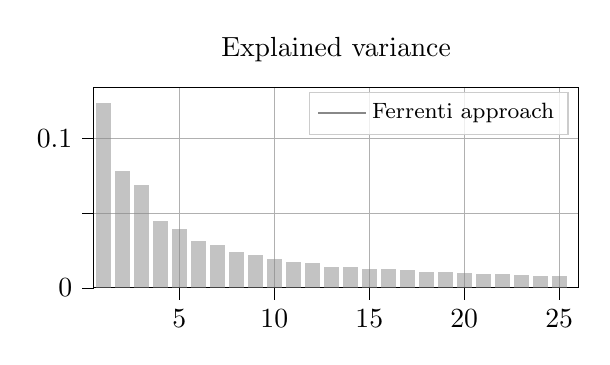
\begin{tikzpicture}

\definecolor{color0}{rgb}{0.8,0.4,0.466666666666667}

\begin{axis}[
height=1.6222438079424382in,
legend style={fill opacity=0.8, draw opacity=1, text opacity=1, draw=white!80!black},
tick align=outside,
tick pos=left,
width=3.0444876158848764in,
x grid style={white!69.0196078431373!black},
xmajorgrids,
xmin=0.5, xmax=26,
xtick style={color=black},
y grid style={white!69.0196078431373!black},
ymajorgrids,
ymin=0, ymax=0.133808014644924,
ytick style={color=black},
yticklabels={, 0, , 0.1},
title={Explained variance},
legend style={font=\footnotesize},
]
\draw[draw=none,fill=white!53.3333333333333!black,fill opacity=0.5] (axis cs:0.6,0) rectangle (axis cs:1.4,0.123808014644924);
\draw[draw=none,fill=white!53.3333333333333!black,fill opacity=0.5] (axis cs:1.6,0) rectangle (axis cs:2.4,0.0779020383908885);
\draw[draw=none,fill=white!53.3333333333333!black,fill opacity=0.5] (axis cs:2.6,0) rectangle (axis cs:3.4,0.0690715494994265);
\draw[draw=none,fill=white!53.3333333333333!black,fill opacity=0.5] (axis cs:3.6,0) rectangle (axis cs:4.4,0.0448634890553009);
\draw[draw=none,fill=white!53.3333333333333!black,fill opacity=0.5] (axis cs:4.6,0) rectangle (axis cs:5.4,0.0396017649392185);
\draw[draw=none,fill=white!53.3333333333333!black,fill opacity=0.5] (axis cs:5.6,0) rectangle (axis cs:6.4,0.0309892340254588);
\draw[draw=none,fill=white!53.3333333333333!black,fill opacity=0.5] (axis cs:6.6,0) rectangle (axis cs:7.4,0.0286471759268761);
\draw[draw=none,fill=white!53.3333333333333!black,fill opacity=0.5] (axis cs:7.6,0) rectangle (axis cs:8.4,0.0241373022722755);
\draw[draw=none,fill=white!53.3333333333333!black,fill opacity=0.5] (axis cs:8.6,0) rectangle (axis cs:9.4,0.0219387724823991);
\draw[draw=none,fill=white!53.3333333333333!black,fill opacity=0.5] (axis cs:9.6,0) rectangle (axis cs:10.4,0.0191941500093896);
\draw[draw=none,fill=white!53.3333333333333!black,fill opacity=0.5] (axis cs:10.6,0) rectangle (axis cs:11.4,0.0170987447716404);
\draw[draw=none,fill=white!53.3333333333333!black,fill opacity=0.5] (axis cs:11.6,0) rectangle (axis cs:12.4,0.0163324377943715);
\draw[draw=none,fill=white!53.3333333333333!black,fill opacity=0.5] (axis cs:12.6,0) rectangle (axis cs:13.4,0.0142479118996461);
\draw[draw=none,fill=white!53.3333333333333!black,fill opacity=0.5] (axis cs:13.6,0) rectangle (axis cs:14.4,0.0139471831901937);
\draw[draw=none,fill=white!53.3333333333333!black,fill opacity=0.5] (axis cs:14.6,0) rectangle (axis cs:15.4,0.0125561362477749);
\draw[draw=none,fill=white!53.3333333333333!black,fill opacity=0.5] (axis cs:15.6,0) rectangle (axis cs:16.4,0.0122752355665442);
\draw[draw=none,fill=white!53.3333333333333!black,fill opacity=0.5] (axis cs:16.6,0) rectangle (axis cs:17.4,0.0117377683648439);
\draw[draw=none,fill=white!53.3333333333333!black,fill opacity=0.5] (axis cs:17.6,0) rectangle (axis cs:18.4,0.0108124054147357);
\draw[draw=none,fill=white!53.3333333333333!black,fill opacity=0.5] (axis cs:18.6,0) rectangle (axis cs:19.4,0.0105912984624588);
\draw[draw=none,fill=white!53.3333333333333!black,fill opacity=0.5] (axis cs:19.6,0) rectangle (axis cs:20.4,0.00987028371434172);
\draw[draw=none,fill=white!53.3333333333333!black,fill opacity=0.5] (axis cs:20.6,0) rectangle (axis cs:21.4,0.00946157777094173);
\draw[draw=none,fill=white!53.3333333333333!black,fill opacity=0.5] (axis cs:21.6,0) rectangle (axis cs:22.4,0.00932051055389097);
\draw[draw=none,fill=white!53.3333333333333!black,fill opacity=0.5] (axis cs:22.6,0) rectangle (axis cs:23.4,0.00851928669553865);
\draw[draw=none,fill=white!53.3333333333333!black,fill opacity=0.5] (axis cs:23.6,0) rectangle (axis cs:24.4,0.00821174057436937);
\draw[draw=none,fill=white!53.3333333333333!black,fill opacity=0.5] (axis cs:24.6,0) rectangle (axis cs:25.4,0.00796122578616887);
\addlegendimage{semithick, color=white!53.3333333333333!black};
\addlegendentry{Ferrenti approach};
\end{axis}

\end{tikzpicture}
